\subsection{Theoretical foundations}
When describing molecules in the framework of quantum mechanics, we are faced with the problem of 
finding solutions to the non-relativistic and time-independent Schrödinger equation
\begin{equation}
    \hat{H} \psi = \Big[- \frac{\hbar^2}{2m} 
        \nabla^2 + \hat{V}(\mathbf{r}) \Big] \psi = E \psi
\end{equation}
where $\psi$ are eigenfunctions of the hamilton operator $\hat{H}$.
It is out of the scope of this introduction to give a complete
and comprehensive introduction into quantum mechanics, therefore
we will not only leave out the most important results, but
furthermore mention those kind of results without proof which
we need for further calculations. For the beginning it is
important to at least write down the characterisic properties
of the harmonic oscillator, in order to perturbate this
kind of potential onto a unharmonic oscillator, which will be
treated with secondorder perturbationtheory. After this we 
immedeatly come to the molecule orbitals, which we need
to resolve the energy levels being measured in this experiment.

\subsubsection{Harmonic oscillator}
The potential for the harmonic oscillator is given as follwing:
\begin{equation}
    \hat{V}= \frac{m}{2} \omega^2 \hat{x}^2
\end{equation}
To solve this equation, the most convenient method is to
introduce different basis of operators resulting in more 
adapted expressions for the energy
~\cite{fliessbach2008quantenmechanik}. We won't derive 
these results here, but rather state the eigenvalues 
(with quantum number $\nu$)
of the energy without proof
(see also figure~\ref{fig:harmonic1}):
\begin{equation}
    H(\nu) = \left ( \nu + \frac{1}{2} \right )\hbar \omega 
    \quad \text{with $\nu\in \mathbb{N_0}$}
\end{equation}
where the wavefunctions are given by
\begin{equation}
    \psi_n(x)= \left(\frac{m\omega}{\pi\hbar}
    \right)^\frac{1}{4}
    \frac{1}{\sqrt{2^nn!}} H_n
    \left(\sqrt{\frac{m\omega}{\hbar}} x \right)
    e^{-\frac{1}{2}\frac{m\omega}{\hbar}x^2}
\end{equation}

and $H_n$ are the Hermite polynomials: 

\begin{equation}
    H_n(x)=(-1)^n e^{x^2}\frac{d^n}{dx^n}\left(e^{-x^2}\right) 
\end{equation}

\begin{figure}[!t]
    \begin{captionbeside}[]{
        Energy levels of the harmonic oscillator with its 
        related wavefunctions\cite{Demtroeder1}.
        }[r]
    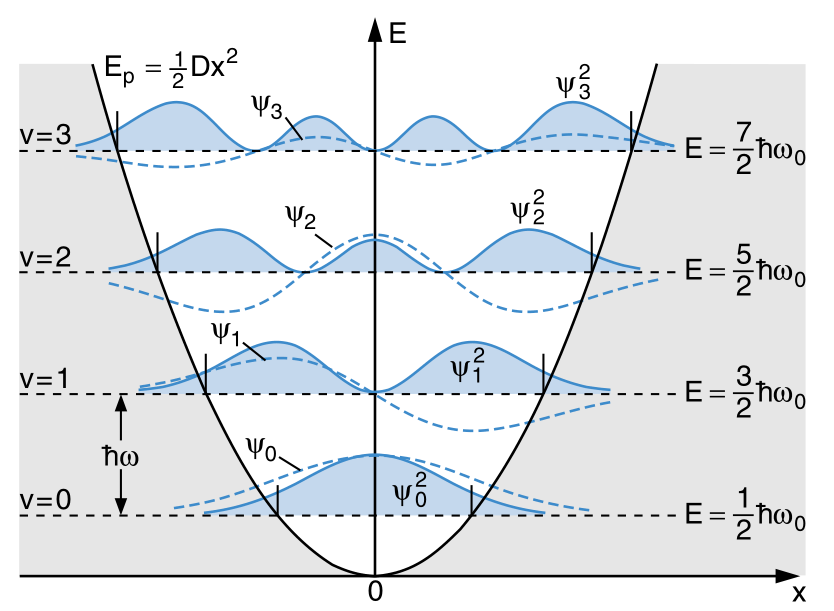
\includegraphics[width=0.65\textwidth]{pics/harmonic1}
    \end{captionbeside}
    \label{fig:harmonic1}
\end{figure}

This potential is of outstanding importance for our experiment,
since the real potential will be aproximated in a region near
the minimum with a harmonic potential. 
For a few problems we can find the analytical solution
to the Schrödinger equation, but in most cases 
we need to approximate the solution with regards to an analyical
solution which is given. In the following sections we will introduce
the time-independent perturbation theory and give an example with the 
anharmonic oscillator of how such an approximation can take place.
\FloatBarrier

\subsubsection{Time-independent perturbation theory}
We are following~\cite{fliessbach2008quantenmechanik}, starting with 
an unpertubed Hamiltonian $\hat{H_0}$ for the harmonic oscillator, 
for which we know the 
eigenstates and -values, numbered with $n\in \mathbb{N}$. 
\begin{equation}
\hat{H_0} |n\rangle = \epsilon_n |n\rangle 
\end{equation}
We further assume the eigenspaces to be
separable, so we have no degeneracy. The case of degeneracy
can be done analogously. 
We search for the solutions of the perturbated Hamiltonian:
\begin{equation}
    \hat{H}|\psi \rangle = E|\psi \rangle 
\end{equation}
by means of the initial Hamiltonian:
\begin{equation}
    \hat{H} = \hat{H_0} + \lambda \hat{V}
\end{equation}
where we perturbate the original Hamiltonian with the potential
$\hat{V}$ and give an approximate solution as long as the perturbation
is not of the same order of magnitude as $H_0$. 
The next step will be to apply this to the anharmonic 
oscillator in order to get an estimation about the energy eigenvalues.
At first we have introduced a new parameter $\lambda$, which is the 
strength of the perturbation; for $\lambda = 1$ we have the problem
we want to solve, for $\lambda = 0 $ we arrive at the unperturbed
problem. Now we can expand in this parameter:
\begin{align}
    E_n(\lambda) &= \epsilon_n + \sum_{\nu =1}^{\infty} \lambda^\nu
    E_{n,\nu} \\ 
    |\psi_n(\lambda)\rangle &=
    |n\rangle + \sum_{\nu =1}^{\infty} \lambda^\nu
    |\psi_{n,\nu}(\lambda)\rangle
\end{align}
As a result, the solutions we are looking for will become:
\begin{align}
    E_n &= \epsilon_n + E_{n,1} + E_{n,2} + \ldots\\ 
    |\psi_n \rangle &= |n\rangle + |\psi_{n,1} \rangle + \ldots 
\end{align}
We assume for now that this series is converging and plug it into
the Schrödinger equation:
\begin{equation}
    (\hat{H_0} + \lambda \hat{V})
   \left( |n\rangle + \sum_{\nu =1}^{\infty} \lambda^\nu
        |\psi_{n,\nu}(\lambda)\rangle \right) =
\epsilon_n + \sum_{\nu =1}^{\infty} \lambda^\nu
    E_{n,\nu}  
    \left( |n\rangle + \sum_{\nu' =1}^{\infty} \lambda^{\nu'}
        |\psi_{n,\nu'}(\lambda)\rangle \right) 
\end{equation}
Now we can impose that the different powers of $\lambda$ have to
match on both sides and receive a set of equations:
\begin{align}
    \hat{H_0} |n\rangle &= \epsilon_n |n\rangle\\
    \hat{H_0} |\psi_{n,1}\rangle + \hat{V}|n\rangle &=
    \epsilon_n |\psi_{n,1}\rangle + E_{n,1}|n\rangle \label{eq:dev1}\\
    \hat{H_0} |\psi_{n,2}\rangle + \hat{V}|\psi_{n,1}\rangle &=
    \epsilon_n |\psi_{n,2}\rangle + E_{n,1}|\psi{n,1}\rangle 
    + E_{n,2}|n\rangle \label{eq:dev2}\
\end{align}
This set of equations yield recursive the solutions of $E_{n,1}$,
$E_{n,2}$ and so on. Now we expand these single wavefunctions 
into the new basis of energy eigenfunctions $|m \rangle$ with $m\in 
\mathbb{N}$:
\begin{equation}
    |\psi_{n,1}\rangle = \sum_{m=1}^{\infty} a_{nm} |m \rangle
    \label{eq:psi_expansion}
\end{equation}
We can plug this expansion into equation~\eqref{eq:dev1}:
\begin{equation}
    \sum_{m=1}^{\infty} (\epsilon_n - \epsilon_m) a_{nm} |m\rangle
    + E_{n,1} |n\rangle = \hat{V}|n \rangle
\end{equation}
With the projection onto the dual eigenstate $\langle k|$ we can
use the orthonormality $\langle k | m \rangle = \delta_{m,k}$ 
of the energy eigenfunctions:
\begin{equation}
     (\epsilon_n - \epsilon_k) a_{nk} 
     + E_{n,1}\delta_{n,k}  = \langle k |\hat{V}|n \rangle
\end{equation}
For the case $k = n$ we get:
\begin{equation}
    E_{n,1} = \langle k |\hat{V}|n \rangle
\end{equation}
and for $k\neq m$:
\begin{equation}
    a_{n,k} = \frac{\langle k |\hat{V}|n \rangle}
    {\epsilon_n - \epsilon_k} \label{eq:a_nk}
\end{equation}
Equation~\eqref{eq:a_nk} together with~\eqref{eq:psi_expansion} 
gives us:
\begin{equation}
    |\psi_{n}\rangle = |n\rangle + \lambda \sum_{m\neq n}^{\infty}
    \frac{\langle m |\hat{V}|n \rangle}{\epsilon_n - \epsilon_m}  
    |m \rangle + \lambda a_{n,n} + \mathcal{O}(\lambda^2)
\end{equation}
Setting $a_{n,n}=0$ (see footnote~\footnote{
Again we can use orthonormality:
\begin{equation*}
    1\overset{!}{=} \langle \psi_n|\psi_{n}\rangle 
    = \left | 1 + \lambda a_{nn} \right |^2 + \lambda^2
    \sum_{m\neq n}^{\infty}
    \left | \frac{\langle m |\hat{V}|n \rangle}
        {\epsilon_n - \epsilon_m} \right |^2 = 
    1 + \lambda (a_{n,n} + a^*_{n,n}) + \mathcal{O}(\lambda^2)
\end{equation*}
When $\lambda > 0 $ this results into:
\begin{equation*}
    a_{n,n} + a^*_{n,n} = 0 \Rightarrow \Re  [a_{n,n}] = 0
\end{equation*}
Since the wavefunctions 
are invariant with respect to a phase $\phi$,
we can set $a_{nn}$ to zero without limitations.} 
for further details), we arrive
at:
\begin{equation}
    |\psi_{n}\rangle = |n\rangle + \lambda \sum_{m\neq n}^{\infty}
    \frac{\langle m |\hat{V}|n \rangle}{\epsilon_n - \epsilon_m}  
    |m \rangle  + \mathcal{O}(\lambda^2)
\end{equation}
For the energy we can make use of the third equation and go to
the second order:
\begin{equation}
|\psi_{n,2}\rangle  = \sum_{m=1}^{X} b_{n,m} |m \rangle 
\end{equation}
We can plug this into equation~\eqref{eq:dev2} analogously and
arrive at:
\begin{equation}
 \sum_{m}^{\infty} (\epsilon_n - \epsilon_m) b_{nm} |m\rangle +
 \sum_{m}^{\infty} E_{n,1} a_{n,m} |m \rangle + E_{n,2} |n \rangle =
 \sum_{m}^{\infty} a_{n,m} \hat{V} |m \rangle
\end{equation}
where we use the orthonormality again. For $k=n$ we get 
\begin{equation}
    E_{n,2} = \sum_{m}^{\infty} a_{n,m} \langle n |\hat{V}|m\rangle
= \sum_{m\neq n}^{\infty}\frac{|\langle n | \hat{V} | m \rangle |^2}
    {\epsilon_n - \epsilon_m}.
\end{equation}
For $k\neq n$ we would arrive at the explicit formula for $b_{n,m}$,
but this is not necessary for further computations considered here.
As a final result we therefore get:
\begin{align}
    E_n &\approx \epsilon_n + \langle n|\hat{V} | n \rangle +
\sum_{m\neq n}^{\infty}\frac{|\langle n | \hat{V} | m \rangle |^2}
    {\epsilon_n - \epsilon_m} \\
    |\psi_n \rangle &\approx 
    |n\rangle + \sum_{m\neq n}^{\infty}
    \frac{\langle m |\hat{V}|n \rangle}{\epsilon_n - \epsilon_m}  
    |m \rangle 
\end{align}


\subsubsection{The anharmonic oscillator}
Lets assume we have solved the harmonic oscillator with 
\begin{align}
    \hat{H_0} &= \frac{\hat{p}^2}{2m} 
    + \frac{1}{2} m \omega_0^2\hat{x}^2 \\
    \hat{H_0}|n \rangle &= \epsilon_n |n \rangle \\
    \epsilon_n &= \hbar \omega_0 \left (n+ \frac{1}{2} \right)
\end{align}
Now perturbe this system with a cubic potential:
\begin{equation}
\hat{V} =\lambda \hat{x}^3
\end{equation}
Hence we can use the perturbation theory in linear order.
Since the parity of $\hat{V}$ is odd, the expectation value has 
to be zero:
\begin{equation}
    E_{n,1} = \lambda \langle n | \hat{x}^3 | n \rangle = 0 
\end{equation}
The wavefunctions have to be corrected as follows:
\begin{eqnarray}
    |\psi_{n,1} \rangle = \sum_{m\neq n}^{\infty}
    \frac{\langle m |\hat{V}|n \rangle}{\epsilon_n - \epsilon_m}  
    |m \rangle 
    = \frac{\lambda}{\hbar \omega}  \\
    |\psi_{n,1} \rangle = \sum_{m\neq n}^{\infty}
    \frac{\langle m |\hat{x}^3|n \rangle}{\epsilon_n - \epsilon_m}  
    |m \rangle 
\end{eqnarray}
We introduce the creation- and annihilation operator 
which are defined by 
\begin{equation}
    \hat{x} = \sqrt{\frac{\hbar}{2m\omega}}(\hat{a}^\dagger +
        \hat{a})
\end{equation} 
and can therefore calculate the matrix elements iteratively
\footnote{
    Here we make use how $\hat{a}$ and $\hat{a}^\dagger$ act 
    on the eigenfunctions $|n\rangle$:
\begin{align*}
    \hat{x}|n'\rangle = \sqrt{\frac{\hbar}{2m\omega}}
    \left ( \sqrt{n' + 1}|n'+1\rangle 
        + \sqrt{n'}|n' - 1 \rangle \right ) 
\end{align*}
Applying once more:
\begin{align*}
\hat{x}^2|n'\rangle = \frac{\hbar}{2m\omega}
\left ( \sqrt{(n' + 1)(n' + 2)}|n'+2\rangle 
            + (2n' + 1) |n' \rangle
            + \sqrt{(n'(n'-1)}|n' - 2 \rangle \right ) 
\end{align*}
And applying for the third time:
\begin{align*}
    \hat{x}^3|n'\rangle &= \sqrt[3]{\left (\frac{\hbar}{2m\omega}\right )^2}
( \sqrt{(n' + 1)(n' + 2)(n'+3)}|n'+3\rangle 
    + 3 \sqrt{(n'+1)^3}|n' +1 \rangle  \\
 &+ 3 \sqrt{(n')^3}|n' -1 \rangle   
            + \sqrt{(n'(n'-1)(n'-2)}|n' - 3 \rangle  ) 
\end{align*}
Now this yields the matrixelements which we need:
\begin{align}
    \langle n | \hat{x}^3 | n' \rangle &=  
    \sqrt{\left (\frac{\hbar}{2m\omega}\right)^3}
( \sqrt{(n' + 1)(n' + 2)(n'+3)}\delta_{n,n'+3} 
    + 3 \sqrt{(n'+1)^3}\delta_{n,n'-1}  \\
    &+ 3 \sqrt{(n')^3}\delta_{n,n'-1}   
    + \sqrt{(n'(n'-1)(n'-2)}\delta_{n,n'-3}  ) 
\end{align}

}. After applying the justified indices, since only $n'=n\pm 1$ and
$m = n \pm 3 $ are not zero, we arrive at:
\begin{equation}
\begin{aligned}
    |\psi_{n,1} \rangle &= \frac{\lambda}{\hbar \omega}
    \sqrt{\left(\frac{\hbar}{2m\omega}\right)^3}
    ( -\frac{1}{3}\sqrt{(n + 1)(n + 2)(n+3)}|n+3\rangle 
    - 3 \sqrt{(n+1)^3}|n +1 \rangle  \\
 &+ 3 \sqrt{(n)^3}|n -1 \rangle  
    +\frac{1}{3} \sqrt{(n(n-1)(n-2)}|n - 3 \rangle  ) 
\end{aligned}
\end{equation}
We can also calculate the energy corrections
\begin{equation}
    E_{n,2} = \langle n | \hat{V} | \psi_{n,1} \rangle 
    = \lambda \langle n | \hat{x}^3 | \psi_{n,1} \rangle 
\end{equation}
which yields
\begin{equation}
\begin{aligned}
    E_{n,2} &= \frac{\hbar^2 \lambda^2}{2 m^3 \omega ^4}
    \left[-\frac{1}{3}(n+1)(n+2)(n+3)
        -9(n+1)^3 + 9n^3 + \frac{1}{3}n(n-1)(n-2)
        \right ] \\
    &= -\frac{\hbar^2 \lambda^2}{2 m^3 \omega ^4}
    \left[ 30n^2+ 30n + 11 \right ]\\
    &= -\frac{30 \hbar^2 \lambda^2}{2 m^3 \omega ^4}
    \left[\left(n + \frac{1}{2} \right)^2 + \frac{11}{30} \right ]\\
\end{aligned}
\end{equation}
If we had a look at the closed form for all orders, we would
notice the possibility to expand the difference in energy in terms
of powers of the original energy $(n+\frac{1}{2})$ which we will
state here without proof:
\begin{equation}
    E_n = \hbar \omega_{0,0} \left(n + \frac{1}{2} \right) 
    - \hbar \omega_{0,1} \left(n + \frac{1}{2} \right)^2  
    + \hbar \omega_{0,2} \left(n + \frac{1}{2} \right)^3  
    + \ldots
\end{equation}
We did not include the small derivation independent of $n$,
since we will look only at differences in energy. Notice that
the final result is only valid for a small, odd perturbation. 


\subsubsection{Energy levels and wavefunctions
    of two-atomic molecules}
First we will write down the full equations of the two-atomic
molecule and investigate afterwards which parts we can further
simplify (the entire derivation will follow \cite{staatsexamen}):
\begin{equation}
        \hat{H}\psi = E\psi 
\end{equation}
where we can expand the Hamiltonian in the position space,
and split it into one part for the electrons ($i$) and another 
for the two nuclei $A$ and $B$:
\begin{equation}
    \hat{H} = \frac{-\hbar^2}{2} 
        \underbrace{\left(
        \sum_{i}{\frac{\nabla_i^2}{m_e}}
        +\frac{\nabla_A^2}{M_A} +\frac{\nabla_B^2}{M_B}
\right)}_{
\substack{\text{kinetic energy}\\\text{of electrons and nuclei}}}
+ \underbrace{\sum_{i>j}{\frac{e^2}{|r_i - r_j|}}
    }_{\substack{\text{potential energy}\\\text{electron-electron}}}
 - \underbrace{\sum_{i}{\frac{Z_A e^2}{|r_i - r_A|}}
 }_{\substack{\text{potential energy}\\\text{electron-nucleon $A$}}}
 - \underbrace{\sum_{i}{\frac{Z_B e^2}{|r_i - r_B|}}
 }_{\substack{\text{potential energy}\\\text{electron-nucleon $B$}}}
 +  \underbrace{\frac{Z_A Z_B e^2}{|r_A - r_B|}
 }_{\substack{\text{potential energy}\\\text{nucleon $A$ - nucleon $B$}}}
\end{equation}
Now we split the solutions for the electrons and nuclei such
that the prior ones change only little when the
distance of the nuclei changes, which is known as the
\textsc{BORN-OPPENHEIMER}-Approximation \cite{staatsexamen}:
\begin{align}
    \psi &= \psi_E ( \ldots r_i \ldots) \psi_N(r_A, r_B) \\
    \hat{ H}_E\psi_E &= \left(- \sum_{i}{\frac{\hbar^2\nabla_i^2}{2m_e}}
    + \sum_{i>j}{\frac{e^2}{|r_i - r_j|}}
    - \sum_{i}\frac{Z_A e^2}{|r_i - r_A|}
    - \sum_{i}\frac{Z_B e^2}{|r_i - r_B|}
    + 
    \right ) \psi_E = 
 E_E \psi_E \\
 \hat{H}_N\psi_N &= \left (
 -\frac{\hbar^2\nabla_A^2}{2M_A} -\frac{\hbar^2\nabla_B^2}{2M_B}
    - \sum_{i}\frac{Z_A e^2}{|r_i - r_A|}
    - \sum_{i}\frac{Z_B e^2}{|r_i - r_B|}
 + \frac{Z_A Z_B e^2}{|r_A - r_B|}
 \right ) \psi_N
=  E_N \psi_N 
\end{align}
Here we fixed the positions for the Hamiltonian
of the electrons such that they are not included in the
wavefunction. The interaction between electrons and the nuclei
will not be neglected since the wavefunctions $\psi_E$ still depend 
on the distance $r$ between the nuclei. 
\par
A problem arises when trying to solve these equations,
since it is not possible without great difficulties. 
The next step is to build up trial solutions of $\psi_E$, 
consisting of of solutions for one-electron-one-nucleon systems. 
These are called one-electron orbital wave
and will be abbreviated
with \textit{MO} (\textit{Molecule orbital}). The trial solutions
will be built up upon linear combinations of of the \textit{MO}
(\textit{Linear combinations of atomic orbitals} method,
\textit{LCAO}). This method was first introduced 1929 by 
Sir John Lennard-Jones and has to be used with caution, since
it is only applicable within certain limits. The parameters appearing 
in these combinations can be constrained by 
expectation values measured in experiments.
We will now turn our attention to the movement of the nuclei.
Since in our case we only have two of them, we can perform 
a coordinate transformation to the center-of-momentum frame with 
a fictional nucleon of mass
\begin{equation}
    \mu = \frac{M_A M_B}{M_A + M_B}
\end{equation}
so that our new Schrödinger equation with the wavefunction of the
fictional nucleon will look like:
\begin{equation}
    \nabla^2 \psi_N + \frac{2\mu}{\hbar^2} 
    \left[ E - V(r) \right] = 0 
\end{equation}
The Laplace operator written in spherical coordinates will yield
the spherical harmonics as eigenfunctions, so we can use a 
seperational ansatz for our wavefunction:
\begin{equation}
    \psi_N(r,\theta,\rho) = \frac{1}{r} S(r)Y(\theta,\rho)
\end{equation}
with the corresponding
differential operator, where $J\in \mathbb{N}_0$
corresponds to the quantum number of the total angular momentum:
\begin{equation}
    \frac{\partial}{\sin\theta \partial \theta}\left (\sin\theta
    \frac{\partial Y}{\partial \theta}\right ) +
\frac{1}{\sin^2\theta} \frac{\partial^2 Y}{ \partial\rho^2}
 + J(J+1)Y = 0
\end{equation}
Thus we can split the rest of the wavefunction into the 
radial component of the operator:

\begin{equation}
    \frac{d^2 S}{dr^2} + \frac{2\mu}{\hbar^2}
    \left ( E - V(r) - \frac{J(J+1)\hbar^2}{2\mu r^2} \right ) S =0 
    \label{eqn:rad_schr}
\end{equation}

If there is no further degeneracy (for instance due to not
considered interactions with the spin of the nuclei) 
we can write down the energy eigenvalues in terms of the 
electron quantum number $n$ and the two further quantum numbers 
$\nu$ and $J$ for vibration and rotation, respectively:
\begin{equation}
    E = E_{n, \nu, J}
\end{equation}
Calculating the eigenvalues analytically is not possible. 
Instead, we do a separational ansatz, writing the approximated hamiltonian 
as a sum of electron, vibrational and rotational energy operators. 
The corresponding wavenumber 
$T$ can then be written as 
    \begin{equation}
    T = T_e(n) + G_n(\nu) + F_{n, \nu}(J), 
    \end{equation}
    where
    \begin{itemize}
    \item $T_e(n)$ is eigenvalue to the electron energy operator 
        with quantum number $n$ ($T_e(1) := 0$);
    \item $G_n(\nu)$ is eigenvalue to the vibrational energy operator 
        with quantum number $\nu$
        for electron state $n$;
    \item $F_{}(J)$ is eigenvalue to the rotational energy operator
        with quantum number $J$
        for electron state $n$ and vibrational state $\nu$.
    \end{itemize} 
This naturally leads to two simplified extrem cases: neglecting either rotation or 
vibration, where the latter is then adjusted for different $\nu$. 


\subsubsection{The rotationless oscillator}
Here we neglect the terms
arising from rotation, which turns out to be opportune looking at the 
length scales of the former calculated eigenvalues.
The operator then becomes:
\begin{equation}
    \frac{d^2 S(r)}{dr^2} + \frac{2\mu}{\hbar^2}
    \left ( E - V(r) )S(r) = 0 \right )
    \label{eqn:V_osc}
\end{equation}
The eigenfunctions and -values depend on the 
potential energy $V(r)$ which for now is unknown. It includes 
the repulsion due to the
Pauli principle of the electron orbits as well as the attraction
of the charges. Furthermore the physical nature of dissociation
of the two nuclei has to be taken into account.
It is not possible to solve the potential analytically. However, 
one can aprroximate $V(r)$ starting with the properties already known:
\begin{itemize}
        \item Pauli principle:
            $\lim\limits_{r \rightarrow 0}{V(r)} = \infty $
        \item Dissociated nuclei:
$\lim\limits_{r \rightarrow \infty}{V(r)} = const. $
\item Before the dissociation: Attraction of the nuclei with
    the maximal attraction at $r_e$ and the dissociation energy
    $D_e$ defined by 
    $ \lim\limits_{r \rightarrow \infty}{V(r)} - V(r_e)=: D_e$ 
\end{itemize}
The idea is now to capture this properties in the coefficients
of the taylored potential and, by doing so, resolving the principle
physical behavior:
\begin{equation}
    V(r) = V(r_e) 
   + \frac{\partial V(r)}{\partial r}|_{r=r_e}(r - r_e)
   + \frac{\partial^2 V(r)}{2!\partial r^2}|_{r=r_e}(r - r_e)^2
   + \frac{\partial^3 V(r)}{3!\partial r^3}|_{r=r_e}(r - r_e)^3
   + \ldots
\end{equation}
As a first approximation for energies near the minimum $r=r_e$ we
can use the harmonic potential. The constant term
$V(r_e)$ can be dropped since we are only interested in 
potential differences.
\begin{equation}
    V_{harm}(r) =
    \frac{\partial^2 V(r)}{2\partial r^2}|_{r=r_e}(r - r_e)^2
    =: \frac{k_e}{2}(r-r_e)^2
\end{equation}
Following this approach we can use the energy eigenvalues of the
harmonic oscillator in order to approximate
the vibrational states $\nu$:
\begin{equation}
    E_\nu =\sqrt{\frac{k_e}{\mu}}\hbar \left (\nu
        + \frac{1}{2}\right )
\end{equation}
In order to chose a more convenient unit we transform this
equation into $\cm$:
\begin{equation}
    G_\mathrm{harm}\left(\nu\right) = \frac{E}{hc} = \omega_0 \left(\nu + \frac{1}{2}\right)
    \quad \text{with the frequency} \quad
    \omega_0 = \frac{1}{2\pi c} \sqrt{\frac{k_e}{\mu}}
    \label{eqn:freq}
\end{equation}
The wider we leave the regime around $r_e$, speaking about 
higher vibrational states, the worse approximation with a harmonic
oscillator becomes. Qualitatively this is the case when energies
come closer to the dissociation energy. An adhoc solution is 
to treat this with the already mentioned perturbation theory in such
a way that we use the condition
\begin{equation}
    \frac{\partial V(r)}{\partial r}|_{r=r_e}        \gg
    \frac{\partial^2 V(r)}{2!\partial r^2}|_{r=r_e}  \gg
    \frac{\partial^3 V(r)}{3!\partial r^3}|_{r=r_e}  
    \ldots
\end{equation}
and can therefore justify the ansatz (see the Dunham expansion
for more details \cite{lefebvre2004spectra}):
\begin{equation}
    G\left(\nu\right) = \omega_e \left(\nu + \frac{1}{2} \right) 
    - \omega_e x_e \left(\nu + \frac{1}{2} \right) ^2 
    + \omega_e y_e \left(\nu + \frac{1}{2} \right) ^3 
    - \omega_e z_e \left(\nu + \frac{1}{2} \right) ^4 
    + \ldots 
    \label{eqn:G(v)_taylor}
\end{equation}
Since in the experiment it is clearly impossible to seperate
the incoming higher frequencies, we will treat $\omega_e x_e$ as 
one variable, similarily to the others, where they also connected
on length scales by
\begin{equation}
    \omega_e \gg \omega_ex_e \gg \omega_e y_e \ldots 
    \label{eqn:gg}
\end{equation}
As before, we can shift the equations to make them more convenient,
in this case defining the energy of the ground level as zero:
\begin{equation}
    G \mapsto G_0 := \left [G-G(0) \right ] 
        \quad \text{which is given by}
    \quad G(0)=\frac{1}{2}\omega_e - \frac{1}{4}\omega_e x_e 
    + \frac{1}{8} \omega_e y_e + \ldots 
\end{equation}
If we now subtract two consecutive terms, we get
\begin{equation}
    \Delta G\left (\nu +\frac{1}{2} \right ) := G(\nu +1 ) - G(\nu) 
    = \omega_e - \omega_e x_e \left (2\nu +2\right ) + \omega_e y_e 
    \left (3\nu^2+ 6\nu + \frac{13}{4} 
        \right) + \ldots 
    \label{eqn:dG1_2}
\end{equation} 
For \eqref{eqn:gg}, one observes that $\Delta G$ plotted over 
$v$ should yield a polynome with an almost linear regime for 
small $v$. This is the bases for the so-called Birge-Sponer 
extrapolation ~\cite{hollas2002basic} for estimating the dissociation energy. 
If we know the approximate quantum number of vibration $\nu_\mathrm{diss}$ 
close to dissociation, we can just sum up the energy levels:
\begin{equation}
    D_0 = \sum_{\nu = 0 }^{\nu_\mathrm{diss}} \Delta G \left (\nu + \frac{1}{2} \right )
    \quad \Rightarrow \quad D_e = G(0) + D_0
    \label{eqn:D_0}
\end{equation}
We have to keep in mind that these methods are merely based on the
assumption that energies should be near the minimal energy at $r_e$.
We can understand that the energy eigenvalues obtained by this
assumption are only valid in this regime, failing in the regime
near the dissociation energy. The logical next step to improve this 
approximation is to look deeper into the form of the potential,
which we will do in the next chapter by introducing the Morse potential.


\subsubsection{Morse potential}
Already in 1929, Phillip McCord Morse proposed an empirical potential
of the form \cite{Demtroeder1}
\begin{equation}
    V(r) = E_B \left[ 1 - e^{-a(r-r_e)}  \right]^2,
\end{equation}
where $E_B$ is the minimum binding energy and $a$ a parameter,
see figure~\ref{fig:Morse}. The parameter is related to the
dissociation energy by 
\begin{equation}
    D_e = \lim\limits_{r \rightarrow \infty}{V(r)}
        = E_B \left[ 1 - \exp(a r_e)  \right]^2
\end{equation}
\begin{figure}[!t]
    \begin{captionbeside}[]{
        Comparison of the Morse and the harmonic potential
        with the real (experimental) potential\cite{Demtroeder1}.
        }[r]
        \includegraphics[width=0.65\textwidth]{pics/Morse_potential}
    \end{captionbeside}
    \label{fig:Morse}
\end{figure}
Fortunatelly it is possible to solve the Schrödinger equation
for the potential analytically. We will shift the energies 
so we will have the following form of the potential:
\begin{equation}
    V(r) = D_e \left[ 1 - e^{-a(r-r_e)}  \right]^2
\end{equation}
The energy eigenvalues for \eqref{eqn:V_osc} can be computed analytically, 
see~\cite{fliessbach2008quantenmechanik}:
\begin{equation}
    E_\nu = h \omega_{e} \left( \nu + \frac{1}{2}
        \right) - \frac{h^2 \omega_{e}^2}{4 D_e} 
    \left( \nu + \frac{1}{2} \right)^2
\end{equation}
where we introduced
\begin{equation}
    \omega_{e} = \sqrt{\frac{a^2 \hbar D_e}{\pi c \mu}}
    \label{eqn:w_e}
\end{equation}
This can be identified directly with the eigenvalues we obtained
from the taylored unharmonic potential. We hereby notice that these
eigenvalues are, since they are connected to the Morse potential,
much more precise with regards to the dissociation energy than
one would expect at the first glance. We can furthermore
find directly a connection between the dissociation energy and 
the paramter $\omega_e$ and by identification of the second
parameter
\begin{equation}
    \omega_e x_e = \frac{\hbar a^2}{4\pi c \mu}
    \label{eqn:wx_e}
\end{equation}
so that we find 
\begin{equation}
    D_e = \frac{\omega_e^2}{4 \omega_e x_e}.
    \label{eqn:D_e}
\end{equation}


\subsubsection{Rotational structure}
The other approximation of \eqref{eqn:rad_schr}
is done by fixing the distance between the two 
nuclei ($r =$const.) such that 
we only look at $V(r)=0$ and $\frac{S(r)}{r} = 1$. We immedeately get
the solutions:
\begin{equation}
    E = \frac{J(J+1)\hbar^2}{2\mu r^2}
\end{equation}
Written in cgs-units, we get the rotational terms
\begin{equation}
    F = \frac{J(J+1)\hbar}{4 \pi \mu c r^2} = B J (J + 1) \quad 
    \mathrm{ with \ } B := \frac{\hbar}{4 \pi \mu c r^2}.
\end{equation}

In order to take into account both rotation and vibration, we expand 
the rotational energy by adding 'elongation terms' $D$:
\begin{equation}
    F = B J (J + 1) - D J^2 (J + 1)^2 + \ldots 
    \qquad \mathrm{where \ } D \ll B
    \label{eqn:E_rot}
\end{equation}
The coefficient $B$ needs to be corrected using the mean distance of 
the nuclei at a corresponding vibrational level $v$, thus 
\begin{equation}
    B_v := \frac{\hbar}{4 \pi \mu c} \overline{\left( \frac{1}{r^2}\right)}_v
\end{equation}
which can subsequently be written in series expansion 
(see \cite{herzberg1950spectra}):
\begin{eqnarray}
    B_v := B_e - \alpha_e \left (v + \frac{1}{2}\right ) 
    \label{eqn:B_v}\\
    B_e := \frac{\hbar}{4 \pi \mu c} \frac{1}{r_e^2}, \quad B_e \gg \alpha_e
    \label{eqn:B_e}
\end{eqnarray}
and a similar expansion for $D$, which in our experiment cannot be resovled 
and will be neglected.


\subsubsection{Transitions of the I2 molecule}
In order to identify the correct transitions of iodine molecule in 
the spectrum of absorbtion, we need to show first theoretically which 
transitions an be observed. 
The states of the iodine molecule is denoted by a combination of 
quantum numbers \cite{herzberg1950spectra}:
\begin{itemize}
    \item the total orbital angular momentum $\Lambda = |M_L|$, where 
        \begin{eqnarray*}
            L_z &=& M_L \hbar \\
            M_L &=& \sum_i (m_l)_i, \\
            M_L &=& L, L - 1, \ldots, -L \\
            |\mathbf{L}| &=& \sqrt{L (L + 1)} \hbar, 
        \end{eqnarray*}
        which is written as $\Sigma, \Pi, \Delta, \Phi, \ldots$ for corresponding 
        $\Lambda = 0, 1, 2, 3, \ldots$;
    \item the multiplicity $(2S + 1)$ where
        \begin{eqnarray*}
            S_z &= \Sigma \hbar \\
            |\mathbf{S}| &=& \sqrt{S (S + 1)} \hbar, 
        \end{eqnarray*}
        with the total electron spin $\mathbf{S}$ precessing around the 
        molecule axis;
    \item the total angular momentum $\Omega = |\Lambda + \Sigma|$;
    \item the parity $u / g$ of the molecule, referring to odd and even, 
        respectively (parity is defined by the eigenvalue of 
        the parity operator, being (-1 / +1), where the parity operator 
        is defined by an inversion of cooridinates);    
    \item the symmetry for reflection through a plan containing the 
        molecular axis $z$, denoted by $+$ and $-$ for conserving or 
        changing the sign applying the corresponding operator.
\end{itemize}
The index $z$ denotes the projection of the operator in question onto the 
molecule axis $z$. In addition, capital letters indicate states with the same 
spin quantum number. The ground state is then labeled $X$, while ascending 
members of exited levels are labeled with $A, B, C, \ldots$. This is justified 
by the selection rules for transition (see below). 
The entire ground state of the iodine molecule can then be written as
\begin{equation}
    X ^1\Sigma_g^+
\end{equation}
where $\Omega = 1$ is ommited. The possible configurations of the exited states 
are given by
\begin{equation}
    ^1\Pi_u, ^3\Pi_{2u}, A ^3\Pi_{u}, B ^3\Pi_{0u}^+, ^3\Pi_{0u}^-,
\end{equation}
where the $\pm$ have been ommited in cases of two-fold degeneracy. 

This is done by applying quantum mechanical 
conservation laws regarding spin and angular momentum. In this case, 
we consider a one-photon transition with not spin-orbit pertubations, 
whose integrated cross section in proportional to
\begin{equation}
    \sigma_{fi}^1 \propto \langle f | \mathbf{\epsilon \cdot \mu} | i \rangle^2
\end{equation}
 where $f$ and $i$ indicate final and initial state, respectivly, 
$\mathbf{\epsilon}$ is the polarization vector of the photon and
$\mathbf{\mu}$ is the electric dipole moment operator. 
The correspoding selection rules due to the symmetry of $\mathbf{\mu}$ 
and in the absence of spin-orbit pertubations 
are given by (ref. to \cite{lefebvre2004spectra}) 
\begin{eqnarray}
    g  \ &\leftrightarrow \ u \\
    \Delta \Lambda \ &=&  \  0, \pm 1 \\
    \Delta \Omega \ &=& \ 0, \pm 1 \\
    \Sigma^\pm \ &\leftrightarrow& \ \Sigma^\pm
\end{eqnarray}
These rules reduce the possible transitions to 
\begin{eqnarray}
    X ^1\Sigma_g^+ &\rightarrow & A ^3\Pi_{u} \quad \mathrm{and} \\
    X ^1\Sigma_g^+ &\rightarrow & B ^3\Pi_{0u}^+, 
\end{eqnarray}
of which the first one shows only $3 - 4\%$ of the intensity of 
the second one. We thus reduce the discussion to the transition 
$X \rightarrow B$. 


The vibrational changes don't require furthers constraints, but the rotational 
modes reduce the possible transitions further. They are given by:
\begin{eqnarray}
    \Delta J \ &=&  \  0, \pm 1 \\
    J = 0 &\nrightarrow& J = 0 \quad \mathrm{forbidden}\\
    \Delta J &=& 0 \quad \mathrm{forbidden \ for \ } \Omega = 0 \leftrightarrow \Omega = 0 \\
    + &\leftrightarrow& - \\
    s &\leftrightarrow& s, \quad a \leftrightarrow a
\end{eqnarray}
As an important consequence for the present case, we observe that only 
transitions with $\Delta J = \pm1$ are allowed. If we rename the rotational 
quantum number $J''$ of the ground level in $J$, we can divide the corresponding 
energy in wavenumbers of a transition into two possible branches with are 
labeled $R$- and $P$-branch for $J = \pm 1$, respectively, following the 
general nomenclature of naming transitions with $\Delta J = \ldots, -2, -1, 0, 1, 2 \ldots$ 
with capital letters $\ldots, O, P, Q, R, S, \ldots$~\cite{lefebvre2004spectra}.
Subtracting \eqref{eqn:E_rot} 
for $\Delta J = \pm1$ yields the corresponding 
energy differences
\begin{eqnarray}
    R(J) &=& \sigma_0 + B_{v'}(J + 1)(J + 2) - B_{v''}J (J + 1) \nonumber \\
         &=& \sigma_0 + 2 B_{v'} + (3 B_{v'} - B_{v''})J + (B_{v'} - B_{v''})J^2 \\
    P(J) &=& \sigma_0 + B_{v'}(J - 1)J - B_{v''}J (J - 1) \nonumber \\
         &=& \sigma_0 - (B_{v'} + B_{v''})J + (B_{v'} - B_{v''})J^2,
\end{eqnarray}
where $\sigma_0$ is the wavenumber resulting from the energy difference in 
$n$ and $\nu$. 
Now we can rename $m:= J+1$ for the R-branch and $m:= - J$ for 
the P-branch in order to express both of these formulas in one:
\begin{equation}
    \sigma = \sigma_0 + (B_{v'} + B_{v''})m
    +  (B_{v'} - B_{v''})m^2
\end{equation}

If $B_{v'} \neq B_{v''}$, we can compute the maximal energy absorped, 
called the \emph{band head}, which is given for 
\begin{equation}
    \frac{\partial \sigma}{\partial m} = 0 
\end{equation}
The solution of this equation is
\begin{equation}
    m_s = \frac{B_{v'} + B_{v''}}{2(B_{v'} - B_{v''})}
\end{equation}
There are two possibilities~\cite{Demtroeder1}:
\begin{itemize}
        \item $B_{v'} < B_{v''} \Leftrightarrow \sigma_\mathrm{head} > \sigma_0$:
            Band head located on the R-branch, thus shifted 
            to the blue side of the rotationless $\sigma_0$ 
            and \emph{shaded to the red}. With \eqref{eqn:B_e} and \eqref{eqn:B_v}, 
            we see immediately that, in this case, $r_e' > r_e''$.
        \item $B_{v'} > B_{v''} \Leftrightarrow \sigma_\mathrm{head} < \sigma_0$:
            Band head located on the P-branch, thus shifted 
            to the red side of the rotationless $\sigma_0$ 
            and \emph{shaded to the violet}, 
            $r_e' < r_e''$.
\end{itemize}
Plotting $\sigma(m)$ yields the so-called Fortrat parabola, which is shown in a 
qualitative manner for the case $B_{v'} < B_{v''}$ in figure \ref{fig:fortrat}.
\begin{figure}
    \centering
    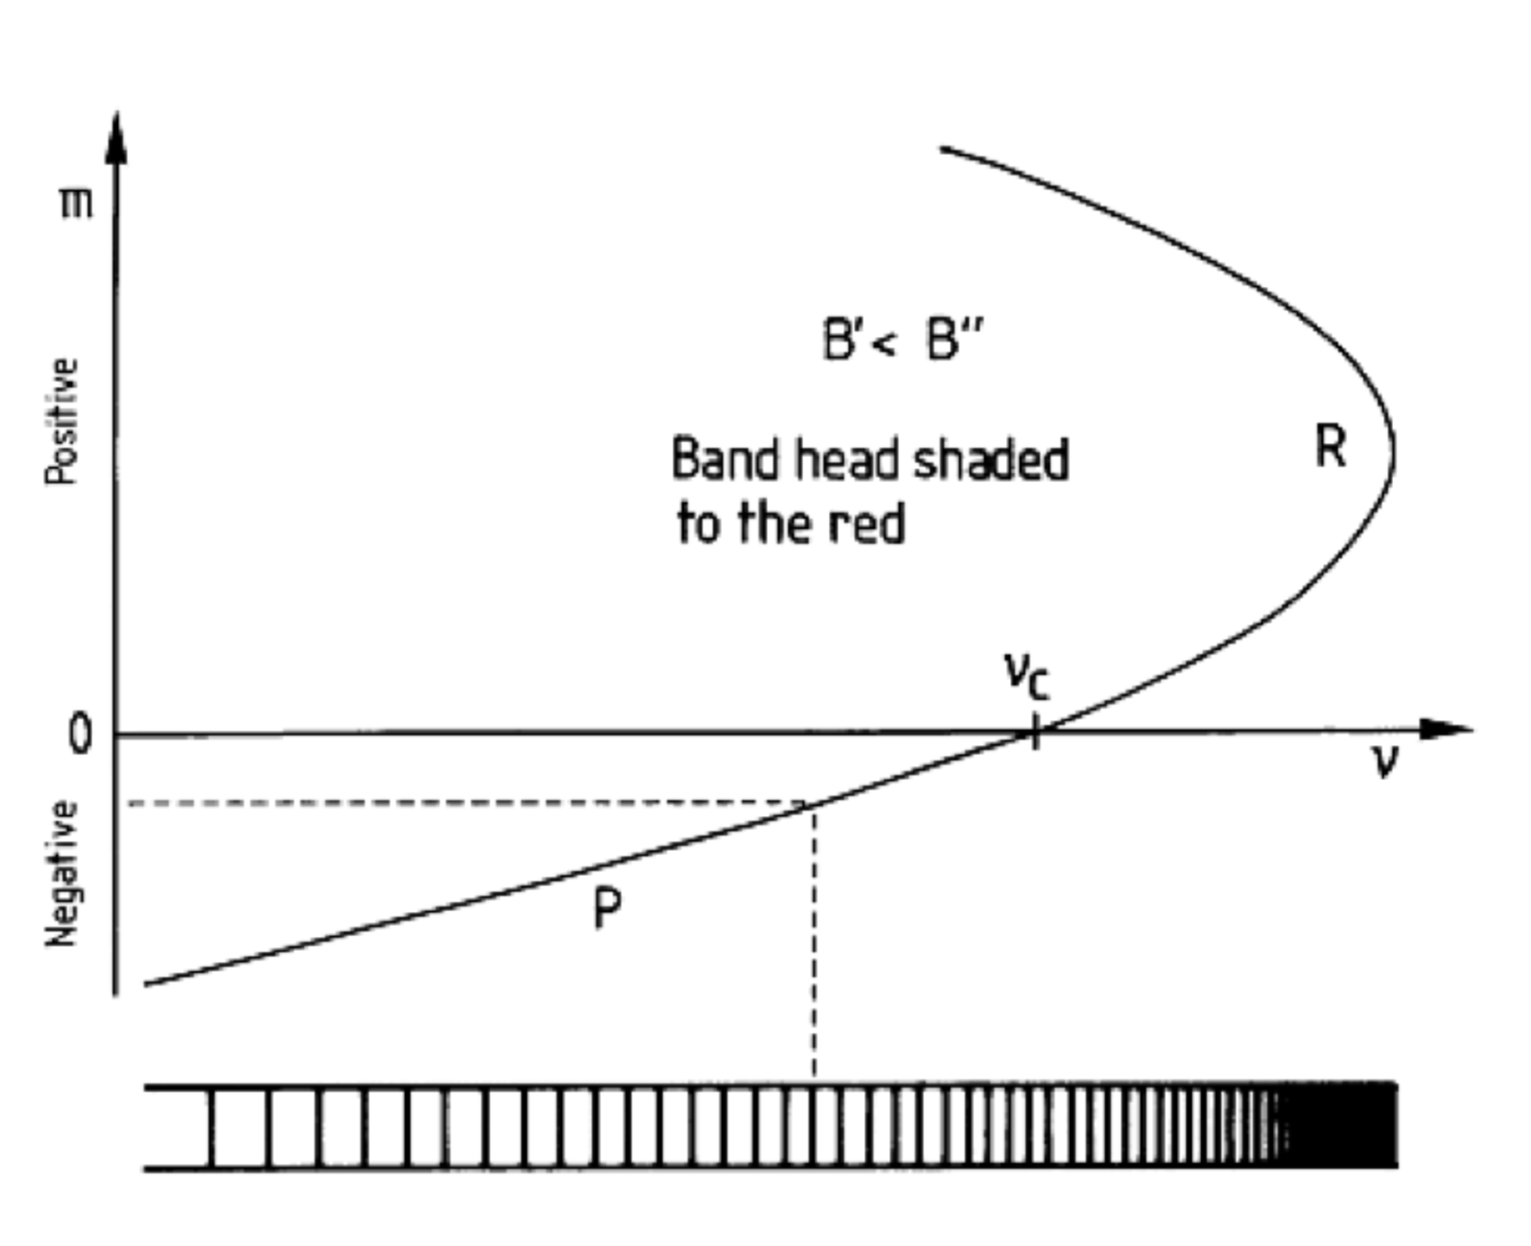
\includegraphics[width=0.6\textwidth]{pics/fortrat.pdf}
    \caption{Fortrat parabola plotting $\sigma(m)$ for a diatomic molecule, where 
    only $P$- and $R$-branch are allowed transitions, corresponding to 
    $\Delta J = -1$, $m = -J$, and $\Delta J = +1$, $m = J + 1$, respectively. 
    The case shown is for $B_{v'} < B_{v''}$, where $\nu_c$ corresponds to the 
    band origin ($J = 0$), the rightmost point of the parabola is the 
    band head shifted to the blue side of $\nu_c$ and the bar below links $m$ to 
    the corresponding $J$. Taken from \cite{Demtroeder1}.
    }
    \label{fig:fortrat}
\end{figure}


If we take literature values~\cite{nist} for the constants, 
\begin{align}
    B_{e}'' &= 0.03737 \ \cm \\ 
    B_{e}'  &= 0.02903 \ \cm \\ 
    \alpha_{e}''  &= 0.000113 \ \cm \\
    \alpha_{e}'  &= 0.000158 \ \cm,
\end{align}
we see, that for the transition under consideration, the band head is shifted 
to the blue side and shaded to the red. Furthermore, we can estimate both the 
difference between band head and \emph{band origin} 
($J = 0$) and the difference between two successive levels, given by
\begin{equation}
    \Delta \sigma := \sigma(m) - \sigma(m-1) = 2 B_{v''} +
    2m(B_{v'} - B_{v''}).
\end{equation}
Using equation \eqref{eqn:B_v}, we get
\begin{eqnarray}
    m_s &\approx& -3 \\
    \sigma_\mathrm{head} - \sigma_0 
        &=& - \frac{(B_v' + B_v'')^2}{4(B_v' - B_v'')} = 0.09 \cm \\
    \Delta \sigma &=& -0.51 \cm \quad (m = 30)
\end{eqnarray}
At a wavelenght of $\lambda_1 \approx \lambda_2 \approx 500\mathrm{nm}$, 
this corresponds to 
\begin{equation}
    \lambda_2 - \lambda_1 = -(\lambda_1 \lambda_2) \Delta \sigma \approx 0.013 \mathrm{nm}.
\end{equation}
Given a resolution of $0.6\nm$, we see that the vibrational states cannot be resolved 
by the spectroscope. We expect a continuosly widened absoprtion peak. The sharpness 
of the peak depends on the distribution of rotational states. As we will not investigate 
the intensity distribution of the absorbtion lines, we will leave out the derivation 
for the statistical distributions for different $n$, $v$ and $J$ as well as the 
Franck-Condon factors for the transitions and refer the reader to the literature, such 
as \cite{lefebvre2004spectra}. 

We can use the given values for $B_e$ to 
perform a calculation of $r_e$, using equation \eqref{eqn:B_e} and 
$\mu m_{I}\/2 \mathrm{u} = 1.05\mathrm{e}-22$g. We get:
\begin{eqnarray}
    r_e   &=& \sqrt{\frac{\hbar}{4 \pi \mu c B_e}} \label{eqn:r_e}\\
    r_e'' &=& 2.675 \AA \label{eqn:r_e0}\\
    r_e'  &=& 3.035 \AA. \label{eqn:r_e1}
\end{eqnarray}
If we look at the potentials drawn from empirical data (figure \ref{fig:i2_pot}), 
we can identify the parameters calculated above:

\begin{figure}[!t]
  \begin{captionbeside}[]{Potential energy curves for the ground state 
    $X ^1\Sigma_{\sigma \, \mathrm{u}}^{+}$ and the first excited state 
    $B ^3\Pi_{\sigma \, \mathrm{u}}^{+}$ of the I2 molecule with examples 
    of wavefunctions for vibrational states $\nu'' = 10$, $\nu'' = 25$ and 
    $\nu' = 26$. Minima of the potentials agree with the radii 
    $r_e'' = 2.675\ \AA$ \eqref{eqn:r_e1} and 
    $r_e'  = 3.035\ \AA$ \eqref{eqn:r_e0} calculated before. 
    Taken from \cite{zare1964calculation}.
    }[r]
    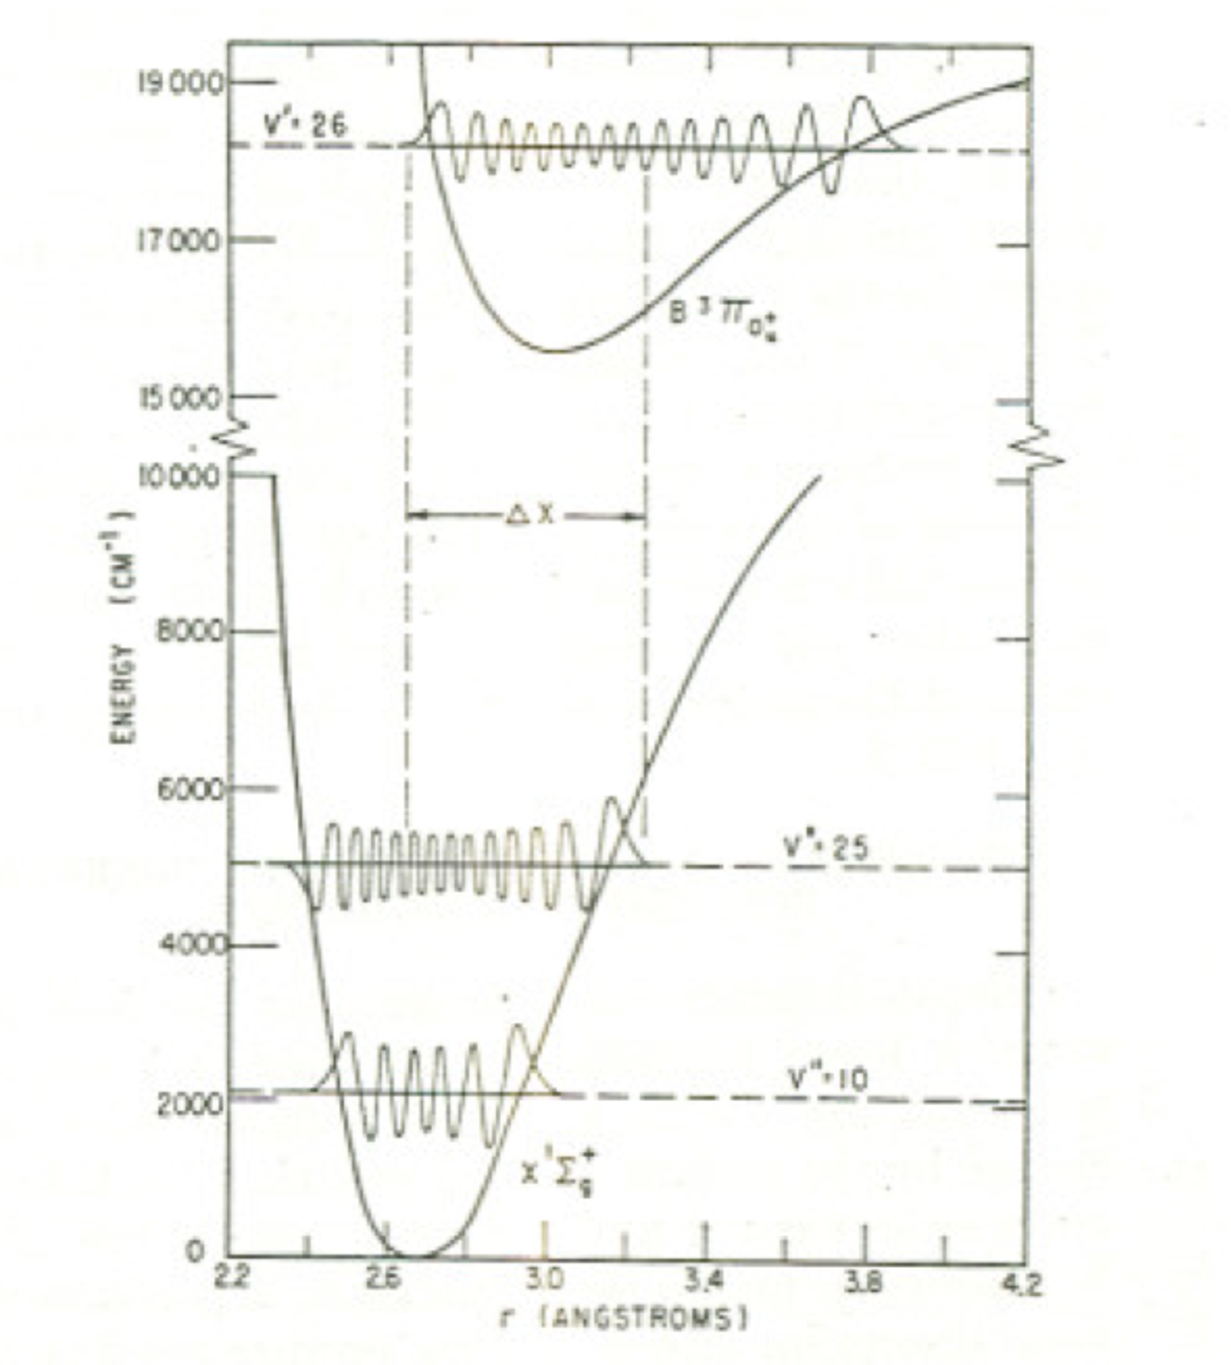
\includegraphics[width=0.65\textwidth]{pics/i2_pot.pdf}
  \end{captionbeside}
    \label{fig:i2_pot}
\end{figure}

Before closing on theoretical preparation, we will state the values for all the 
parameters in question as they are given in literature in table \ref{tab:lit_val}.
In figure~\ref{fig:i2_pot2}, the different energies are shown according to their 
definitions. 

\begin{table}[h]
    \centering
    \begin{tabular}{|l |l |}
        \hline
        Ground state $X ^1\Sigma_{\sigma \, \mathrm{u}}^{+}$ & 
        Excited state $B ^3\Pi_{\sigma \, \mathrm{u}}^{+}$ \\ \hline
        $\omega_e'' = 214.50 \cm    $ & $\omega_e' = 125.69 \cm             $  \\ \hline
        $\omega_e x_e'' = 0.614 \cm $ & $\omega_e x_e' = 0.764 \cm          $  \\ \hline
        $                           $ & $\omega_e y_e' = -0.00567 \cm ^*    $  \\ \hline
        $ D_e'' = 12453 ^{**}$      & $ D_e' = 4391.0 \cm ^*                $  \\ \hline
        $ B_e'' = 0.03737           $ & $ B_e' = 0.02903                    $  \\ \hline
        $ \alpha_e'' = 0.000113     $ & $ \alpha_e' = 0.000158              $  \\ \hline
        $ r_e'' = 2.666 \ \AA       $ & $ r_e' = 3.024 \ \AA                $  \\ \hline
        $ T_e'' = 0 \cm             $ & $T_e' = 15769.01 \cm                $ \\ \hline
    \end{tabular}
    \caption{Literature values for some characteristic parameters of the I2 molecule.
    Values without any marker are taken from \cite{nist}, 
    those marked by $^*$ from \cite{steinfeld1965spectroscopic} and 
    those marked by $^{**}$ from \cite{leroy1970spectroscopic}.}
    \label{tab:lit_val}
\end{table}

\begin{figure}
    \centering
    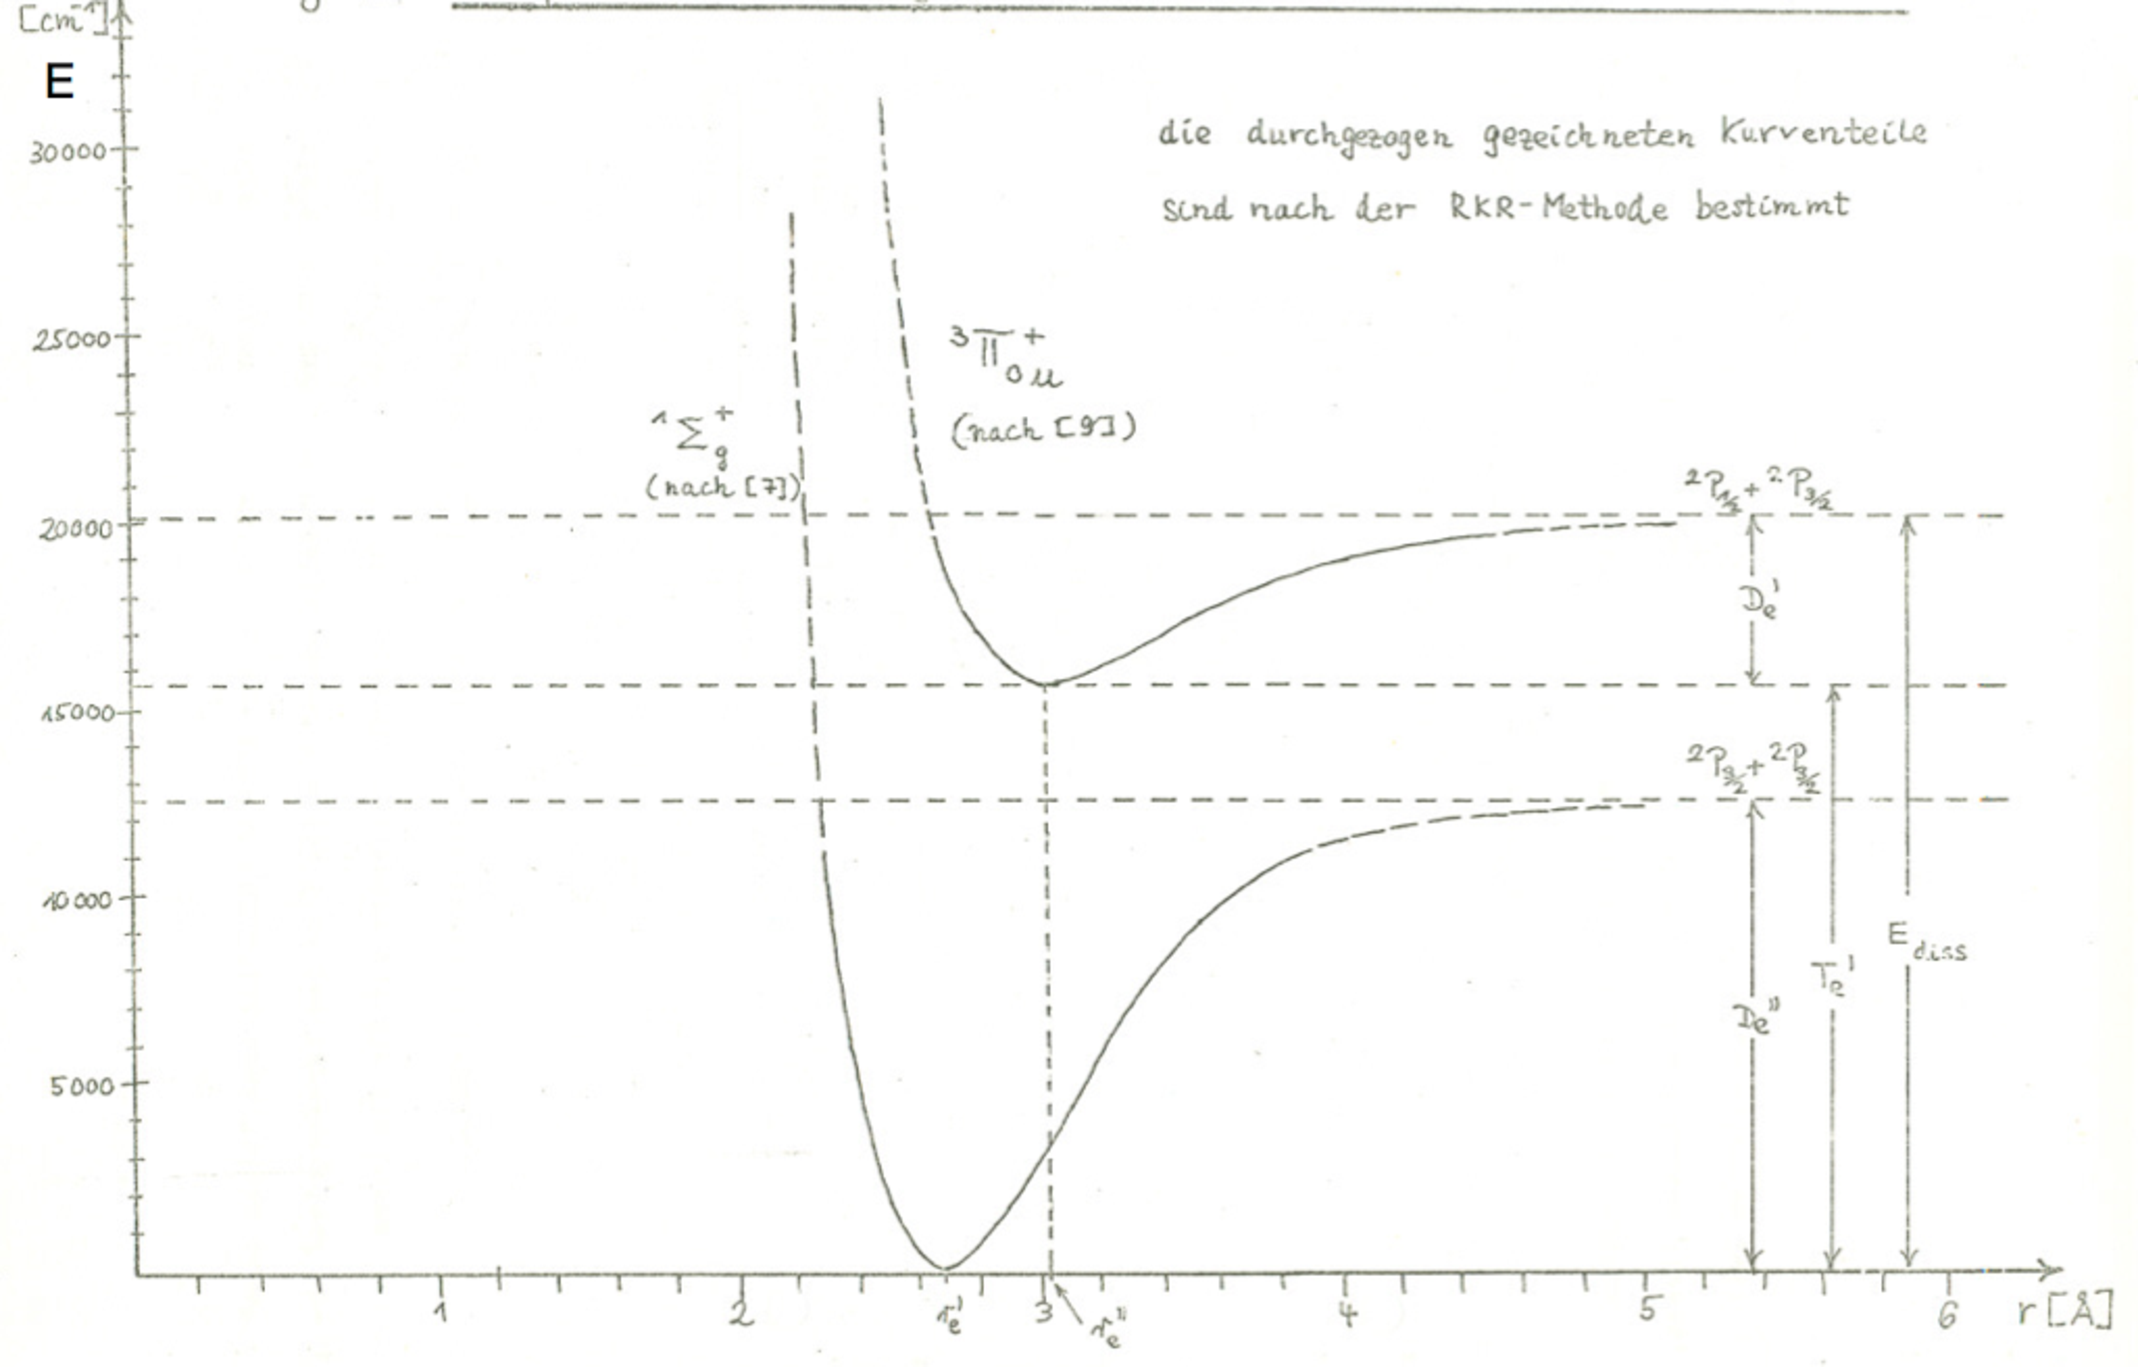
\includegraphics[width=1.0\textwidth]{pics/i2_pot2.pdf}
    \caption{Potential energy curves for thr ground state and the first excited 
    state, including the various differences in energy defined in this section. 
    The continuous lines are derived by the Rydberg-Klein-Rees method (here not 
    further described, see \cite{zare1964calculation} for a description). 
    Taken from \cite{staatsexamen}.}
    \label{fig:i2_pot2}
\end{figure}

\FloatBarrier
